\section{Milestone I}\label{M1}
In this section we want to study the evolution of the uniform background in the Universe. Our main goal of this section will be to implement methods that computes the Hubble parameter, as well as related time- and distance measures \note{Rewrite}. To do this, we will solve \note{simple} ordinary differential equations (ODEs) numerically. For the fiducial cosmology we will use results from \cite{Planck2020}. We will then test our implementation with known theoretical solutions, to assess the validity of our methods. 

The main goal of this section is mainly concerned with using known parameter values to \note{predict/solve} the background cosmology. Another interesting aspect is to use data to constrain such cosmological parameters. To do this, we will use data from supernova observations \cite{Supernova2014Betoule}, containing luminosity distance associated with different values of redshift. Implementing our solver, we will implement a simple Markov chain Monte Carlo (MCMC) algorithm, in order to estimate the best fits of $h,\,\Omega_m$ and $\Omega_\Lambda$, which are the Hubble parameter, and the density parameter of matter and dark energy, respectively.   


\subsection{Theory}\label{M1:theory}
The theory behind this milestone. \note{Define ALL parameters}

\note{Neutrinos are on the loose. Catch them before it's too late.}

When we don't assume $k=0$ and omit neutrino contribution, i.e. setting $\onun=0$, the Friedmann equation can be written as 
\begin{equation}
    H = H_0 \sqrt{\omn a^{-3} + \ogn a^{-4} + \okn a^{-2} + \oln}, \label{M1:theory:eq:Friedmann_H_omegas}
\end{equation}
where $H\equiv\dot{a}/a$ is the Hubble parameter. Dot denotes a derivative with respect to cosmic time, $t$. The matter component is the sum of the baryon and cold dark matter (CDM) components, $\omn=\obn+\ocdmn$. We also introduce the scaled Hubble factor, $\H\equiv aH$. Rather than working with the scale factor, $a(t)$, we will be working with the logarithm of the scale factor 
\begin{equation} \label{M1:theory:eq:x_dx_definitions}
    x\equiv \ln a,\quad '\equiv \dv{x}. 
\end{equation}
%
%
The resulting expression for $\Hx$ is thus  
\begin{equation} \label{M1:theory:eq:Hp_of_x}
    \Hx = H_0 \sqrt{\omn e^{-x} + \ogn e^{-2x} + \okn + \oln e^{2x}}. 
\end{equation}
%
%
We will need the first and second derivative of $\Hx$. To simplify the resulting expressions, we define the function, $g(x)$, as the derivative of the term inside the square root in Eq. \eqref{M1:theory:eq:Hp_of_x}, namely 
\begin{equation}
    g(x) \equiv -\omn e^{-x} -2\ogn e^{-2x} + 2\oln e^{2x}. \label{M1:theory:eq:g_of_x} 
\end{equation} 
%
Using the chain rule, the first two derivatives of $\Hx$ can be written as 
\begin{align} 
    \dv{\H(x)}{x} &= \frac{H_0^2}{2\Hx}g(x), \label{M1:theory:eq:dHp_dx} \\
    \dv[2]{\Hx}{x} &= \frac{H_0^2}{2\Hx}\bracket{g'(x) - \frac{1}{2}\closed{\frac{H_0 g(x)}{\Hx}}^2}. \label{M1:theory:eq:ddHp_ddx}
\end{align}


\begin{align}
    \ok(x) &= \frac{\okn}{\Hx^2 / H_0^2}, \\ 
    \om(x) &= \frac{\omn}{e^x \Hx^2 / H_0^2}, \\ 
    \og(x) &= \frac{\ogn}{e^{2x} \Hx^2 / H_0^2}, \\ 
    \ol(x) &= \frac{\oln}{e^{-2x} \Hx^2 / H_0^2}, \\    
\end{align}

The density parameter of the photons today, $\ogn$, is given by 
\begin{equation}
    \ogn = 2 \cdot \frac{\pi^2}{30} \frac{(k_b T_\mathrm{CMB0})^4}{\hbar^3 c^5} \cdot \frac{8\pi G}{3H_0^2}, \label{M1:theory:eq:omega_gamma0_T}
\end{equation}
where $T_\mathrm{CMB0}$ denotes the temperature of the CMB today. 


\subsection{Implementation details}\label{M1:implementation} 
Something about the numerical work.

\subsection{Results}\label{M1:results}
\subsubsection{Sanity checks}
Show and discuss the results.



\begin{figure}
    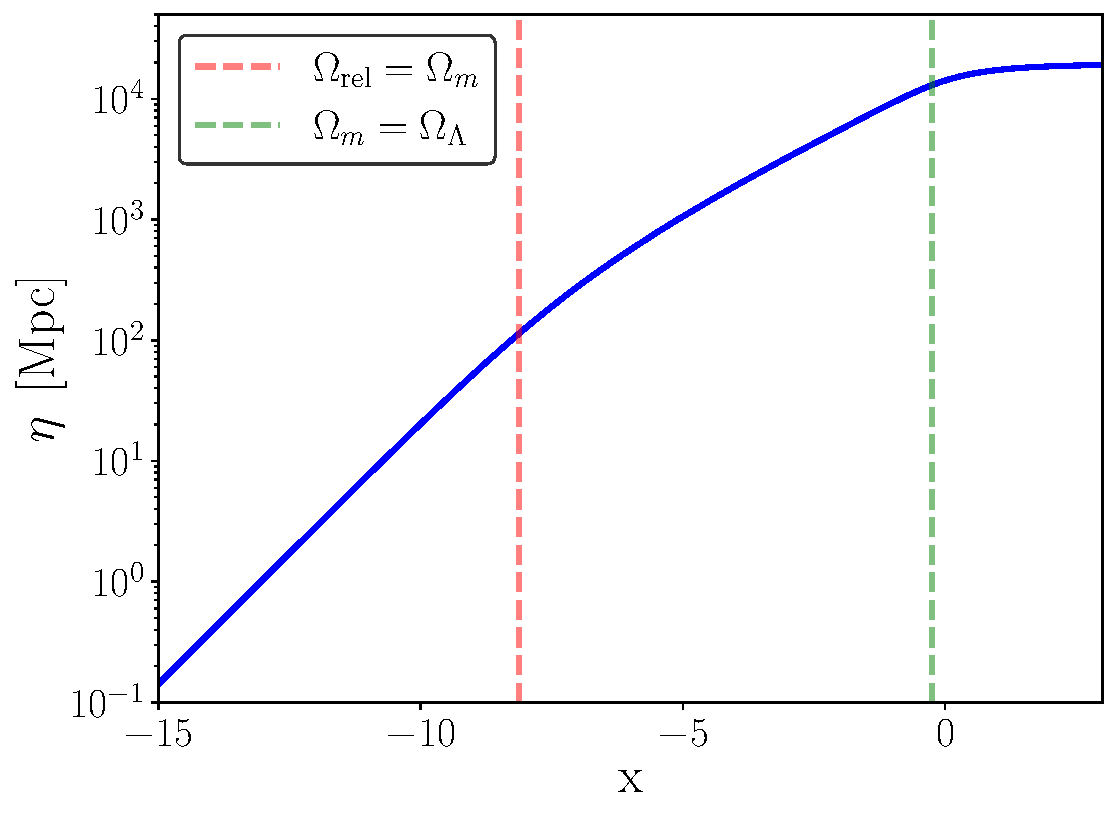
\includegraphics[width=\linewidth]{compare_eta.pdf}
    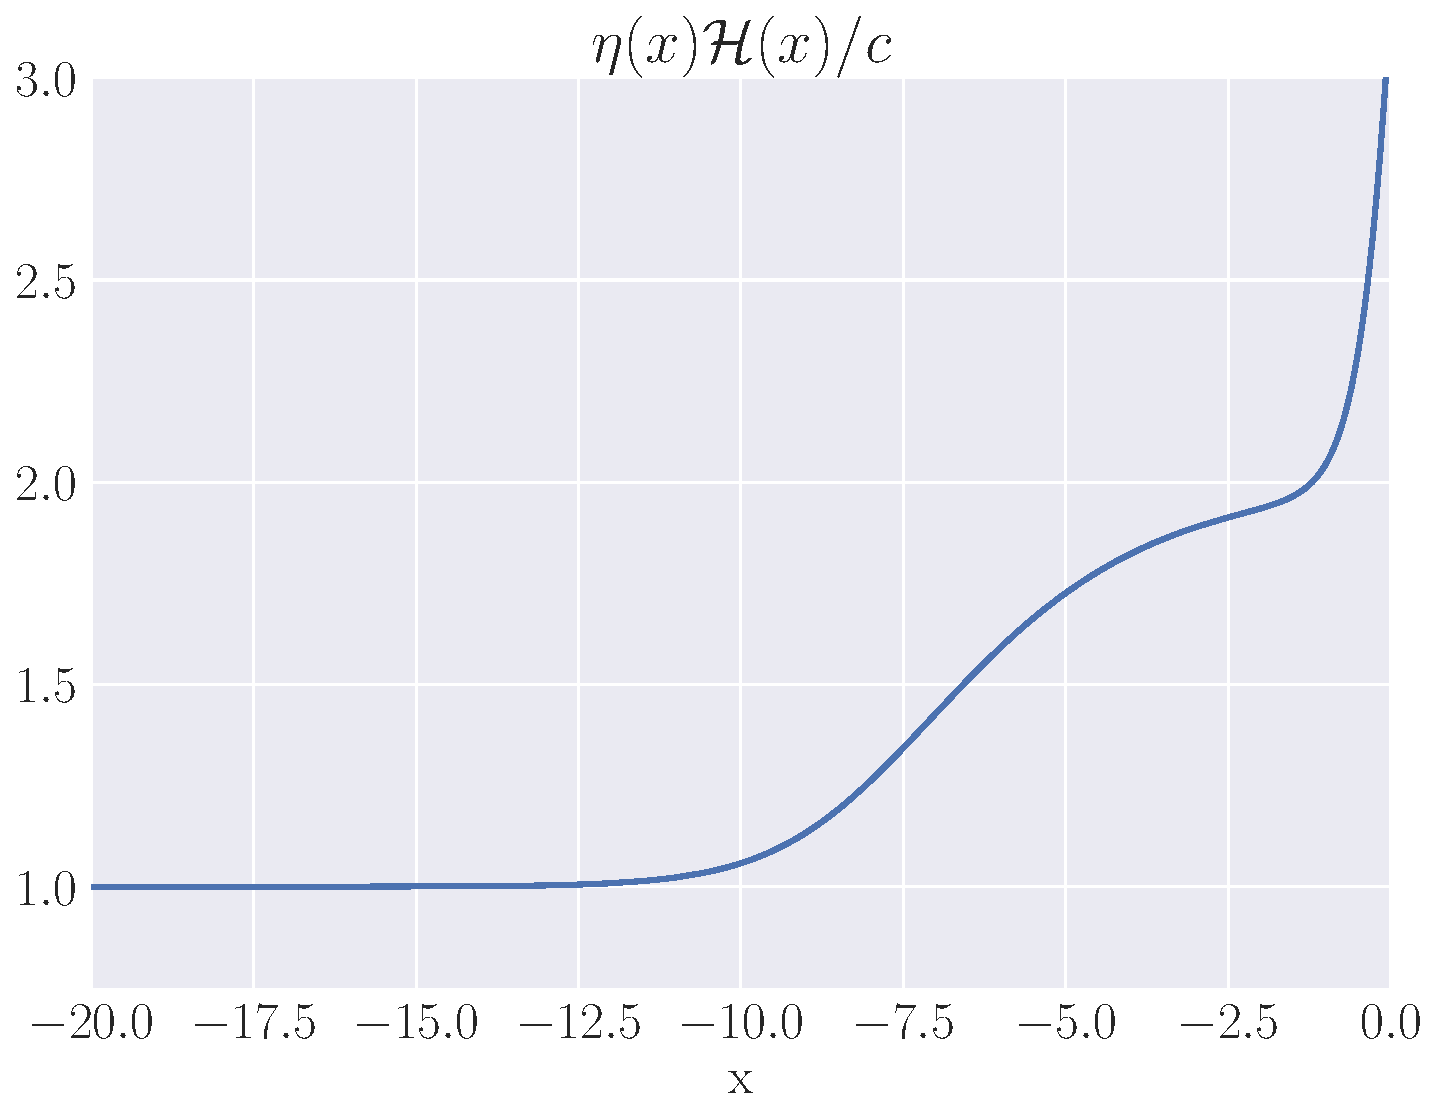
\includegraphics[width=\linewidth]{compare_eta_H_over_c.pdf}
    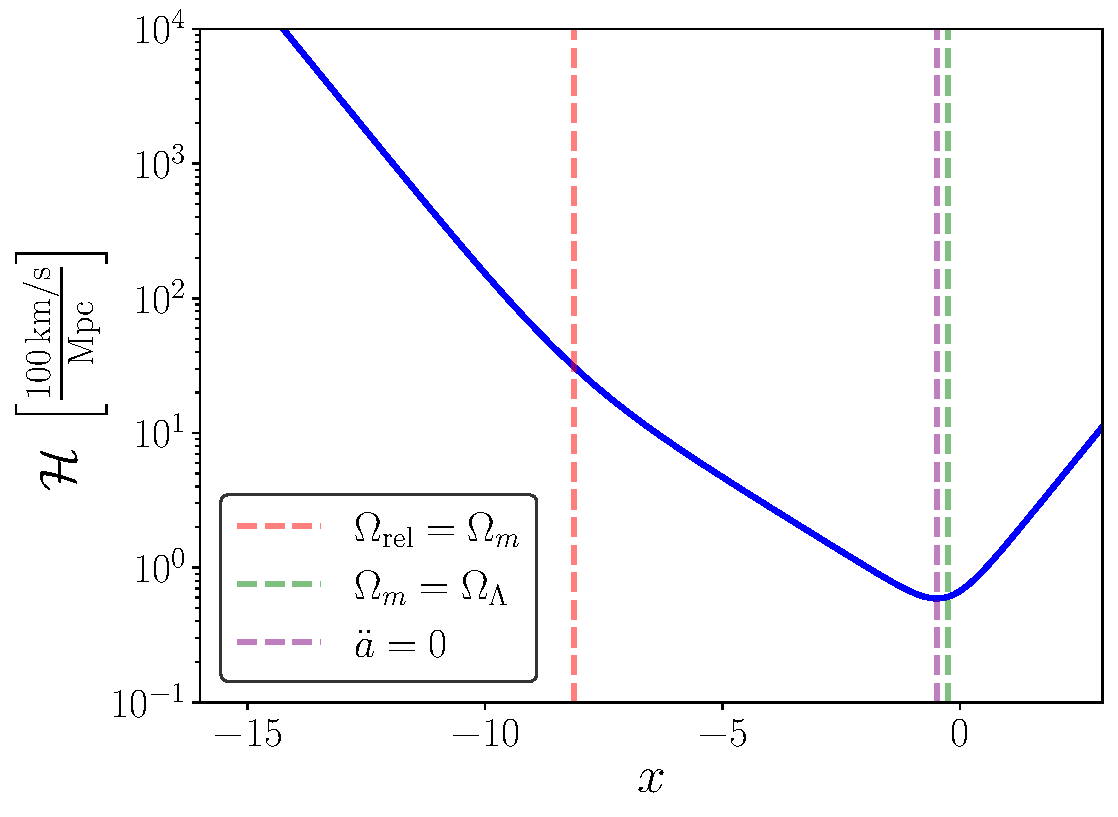
\includegraphics[width=\linewidth]{compare_Hp.pdf}
\end{figure}

\begin{figure}[ht!]
    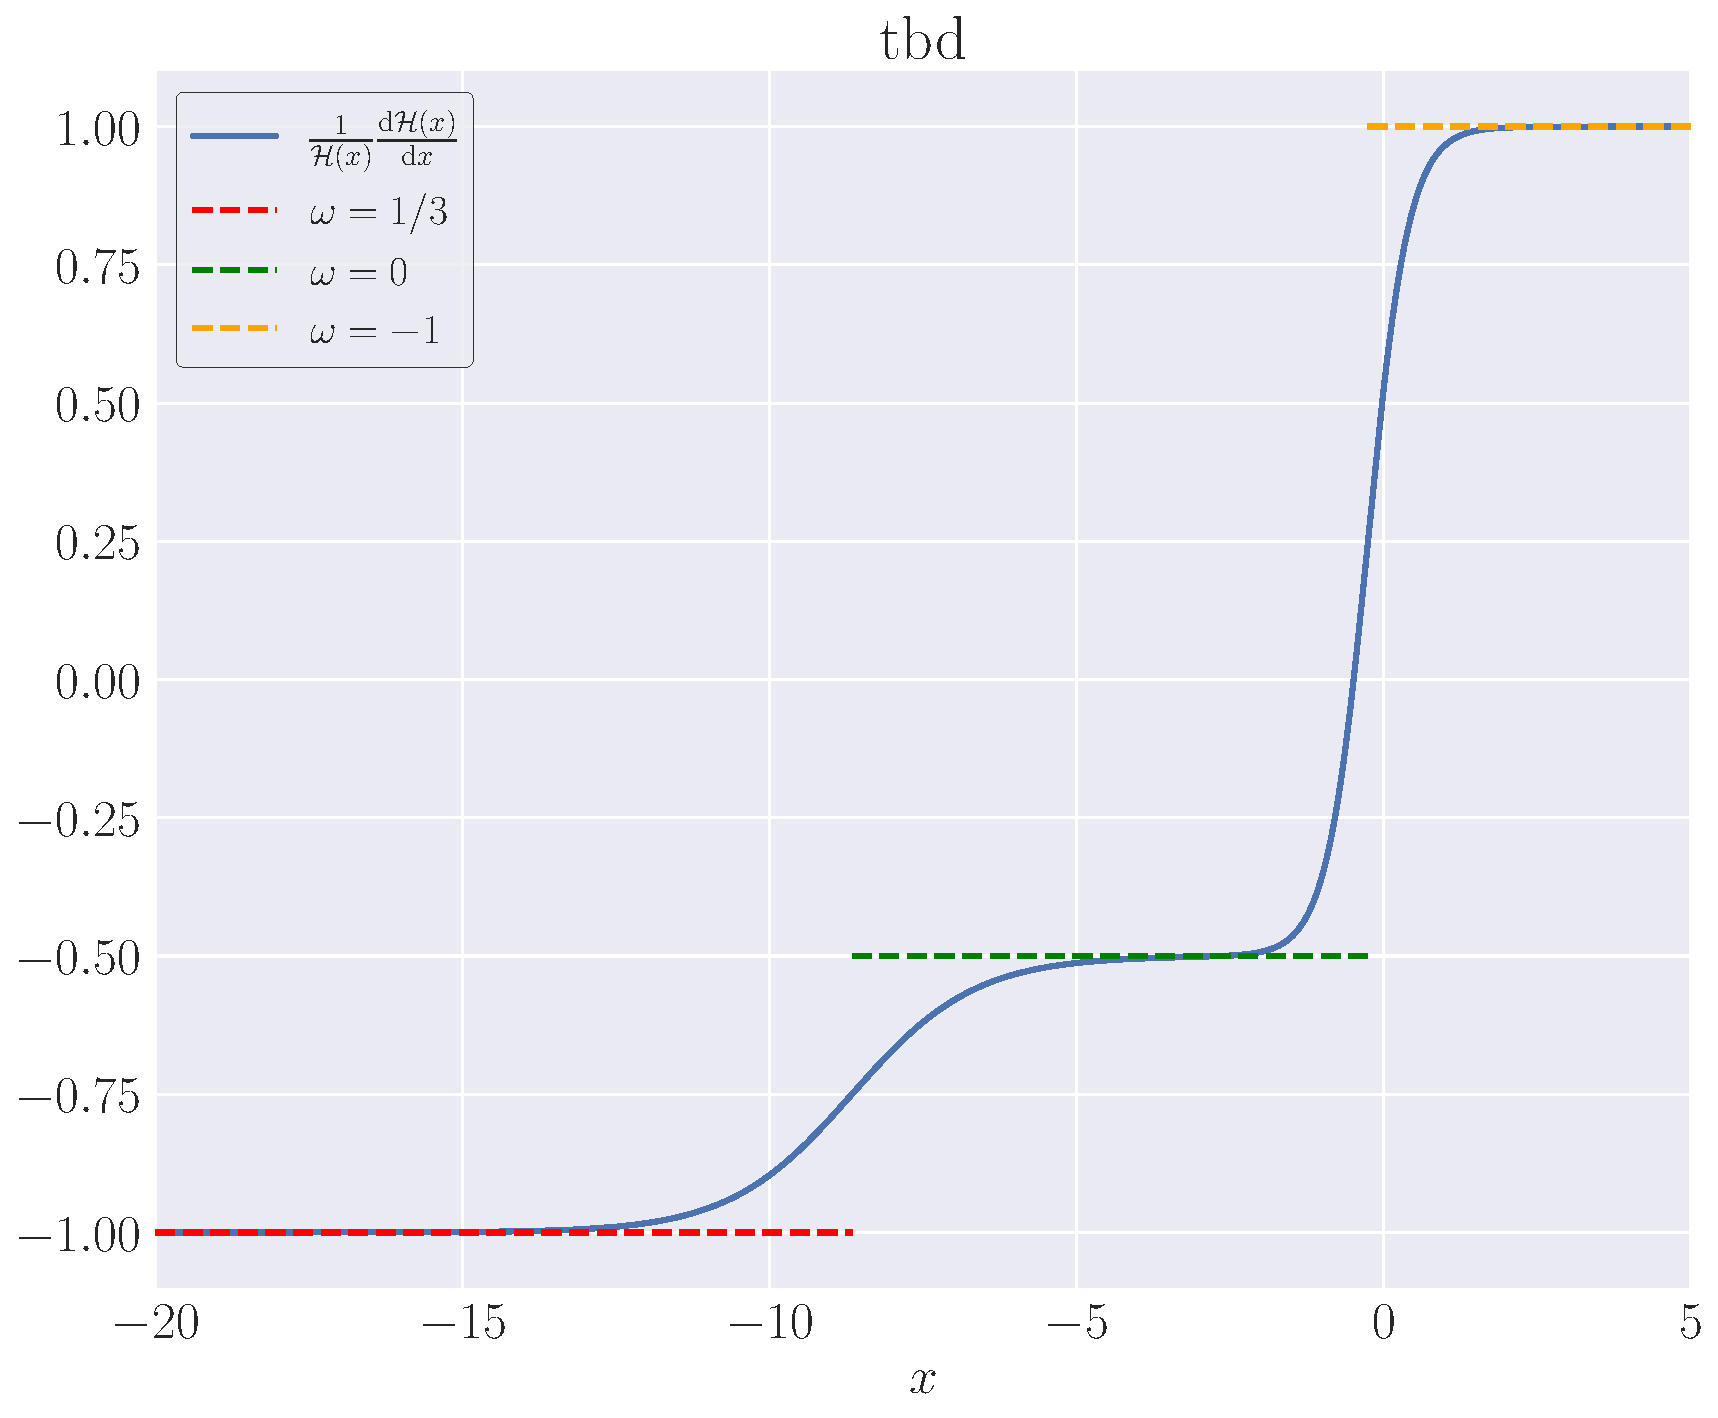
\includegraphics[width=\linewidth]{dH_over_H.pdf}
    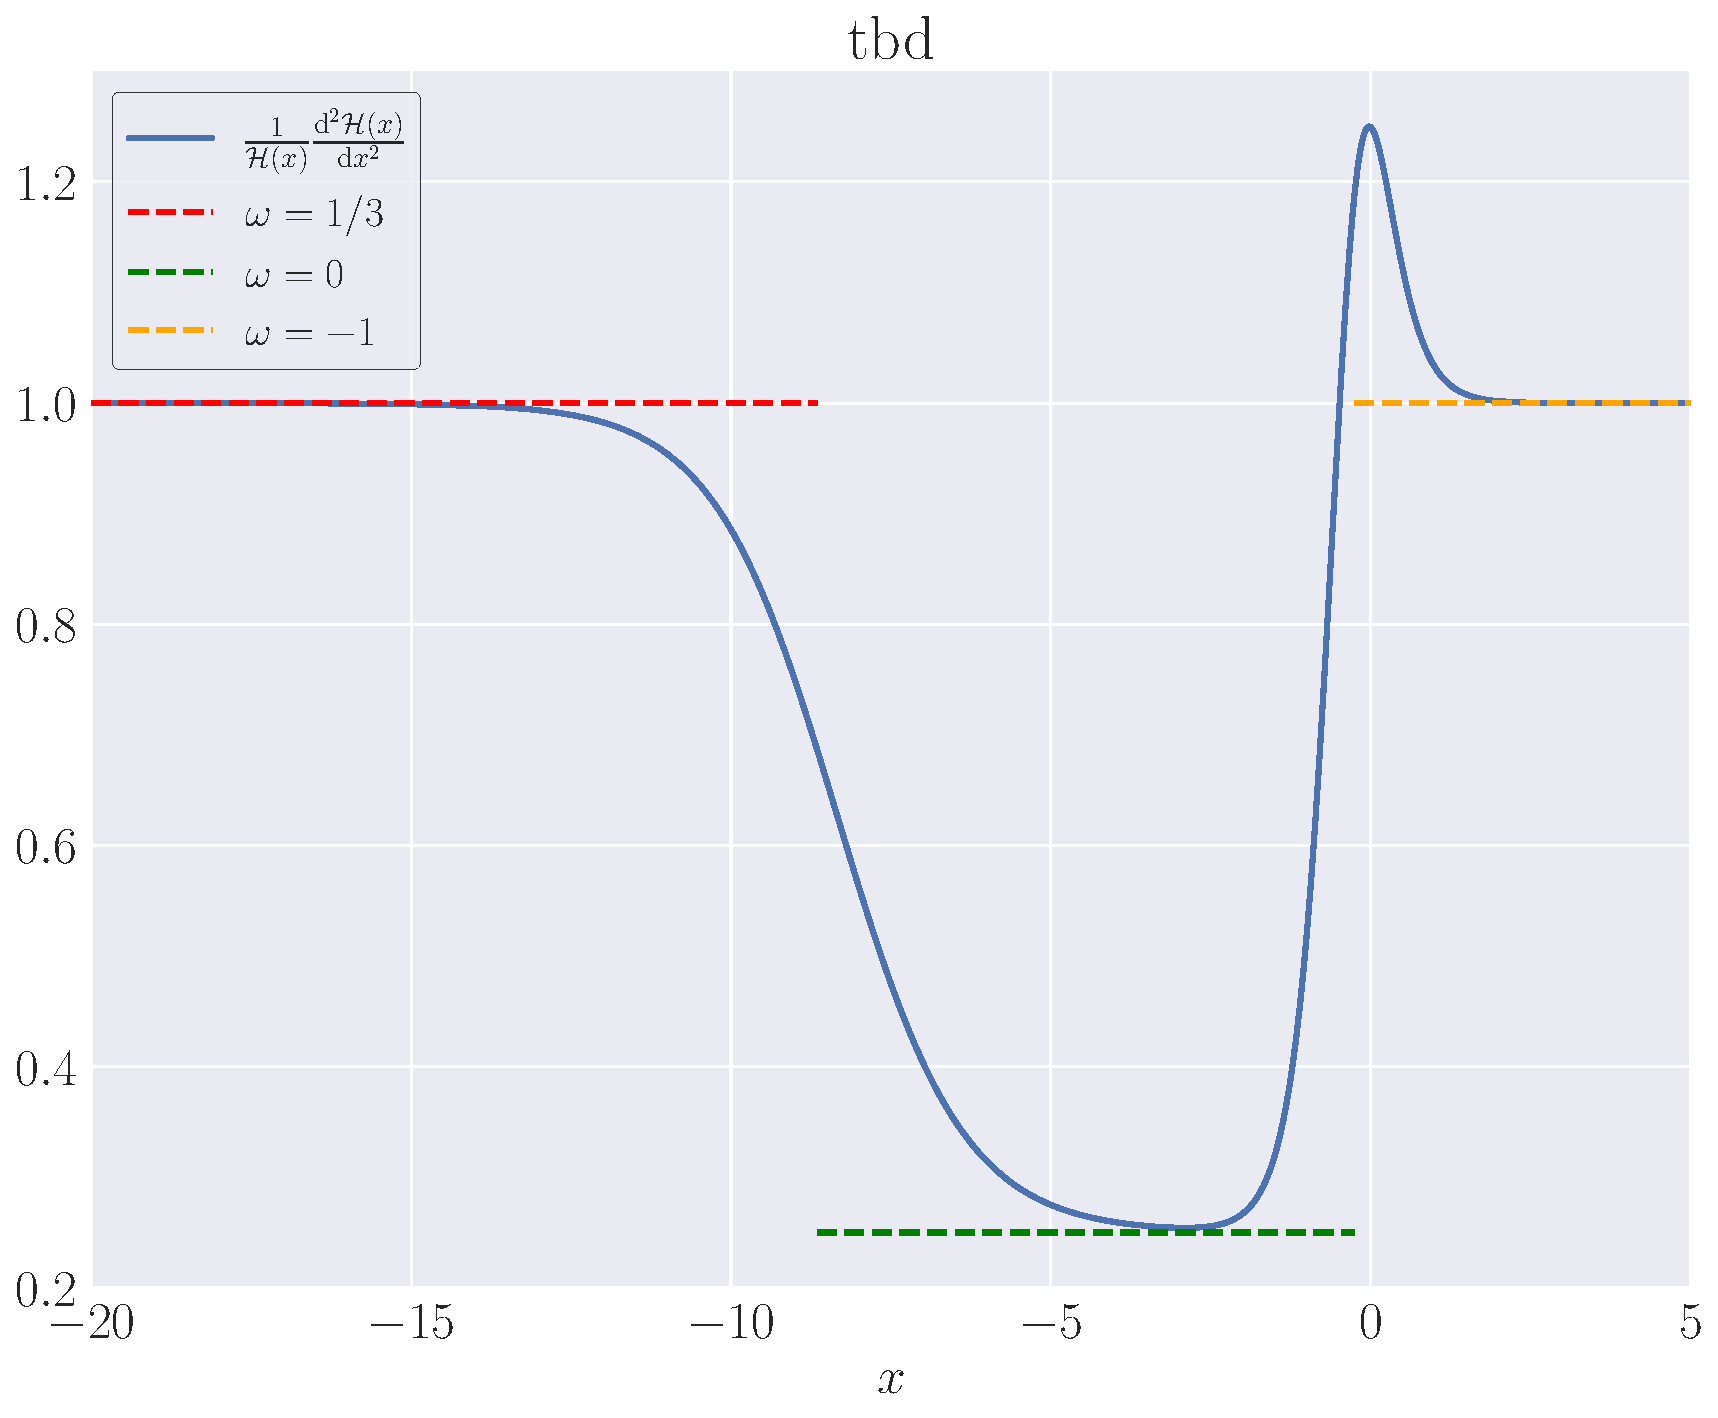
\includegraphics[width=\linewidth]{ddH_over_H.pdf}
\end{figure}

\begin{figure}[ht!]
    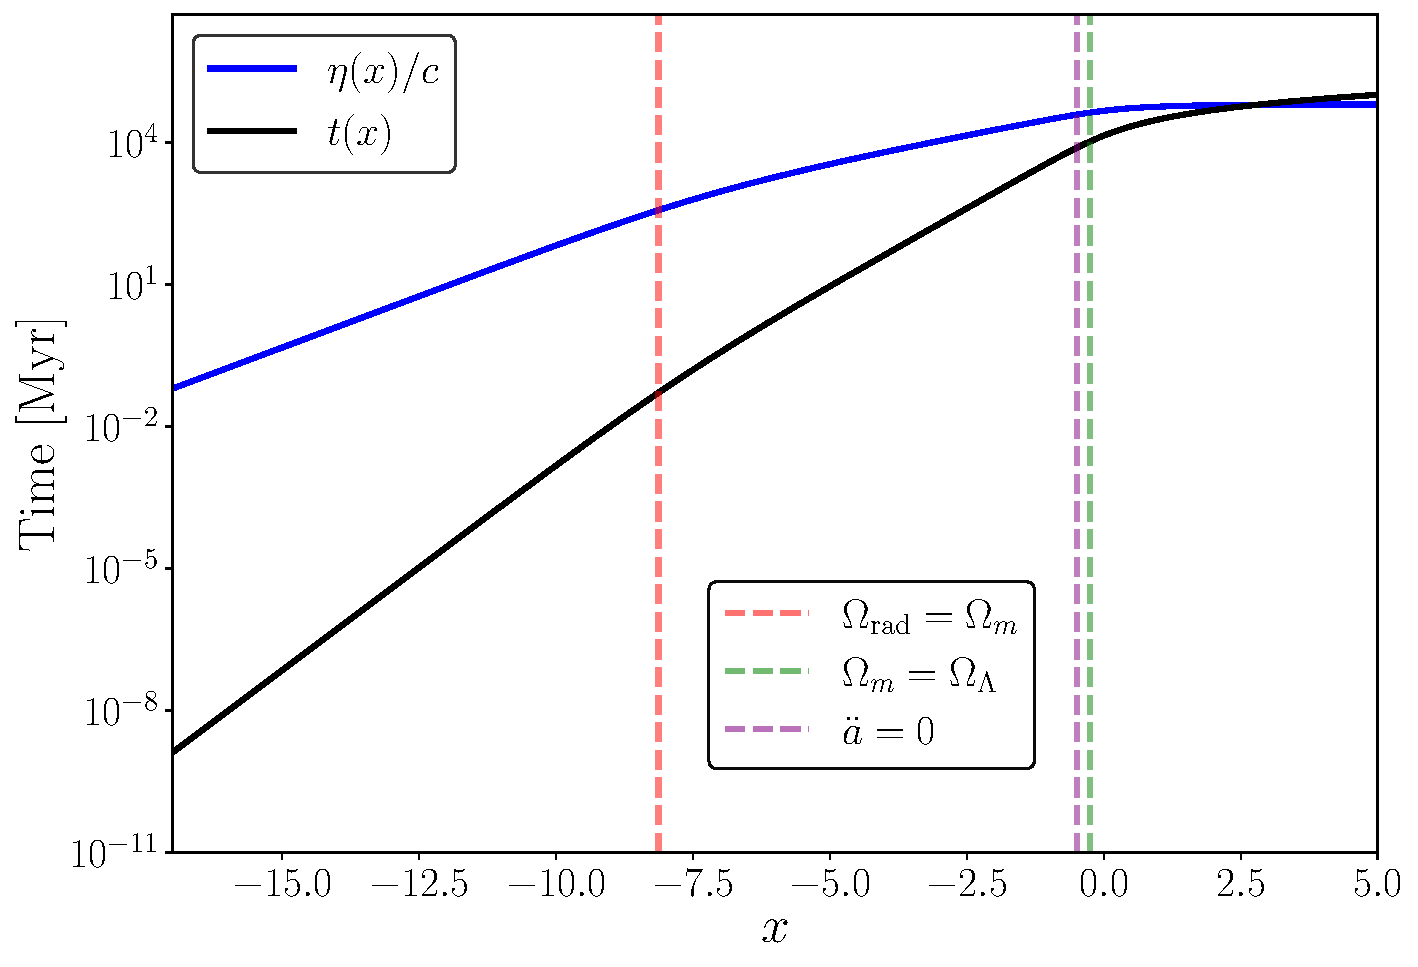
\includegraphics[width=\linewidth]{t_and_eta_c.pdf}
\end{figure}


\begin{figure}[ht!]
    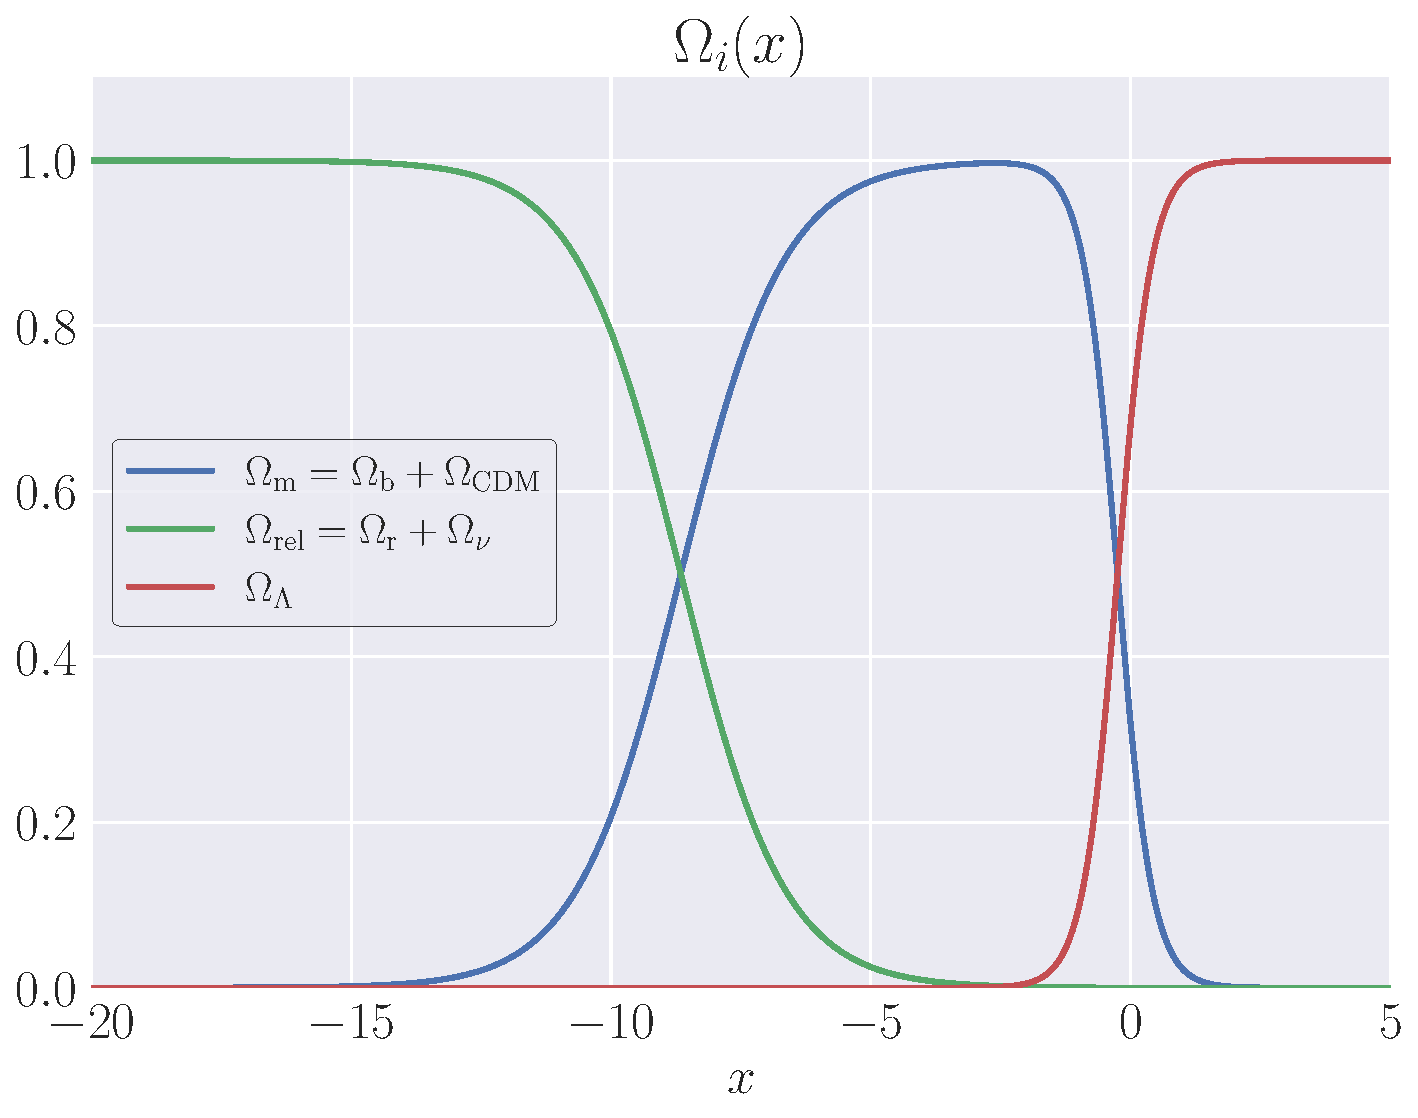
\includegraphics[width=\linewidth]{omega_i_of_x.pdf}
\end{figure}

\begin{figure}[ht!]
    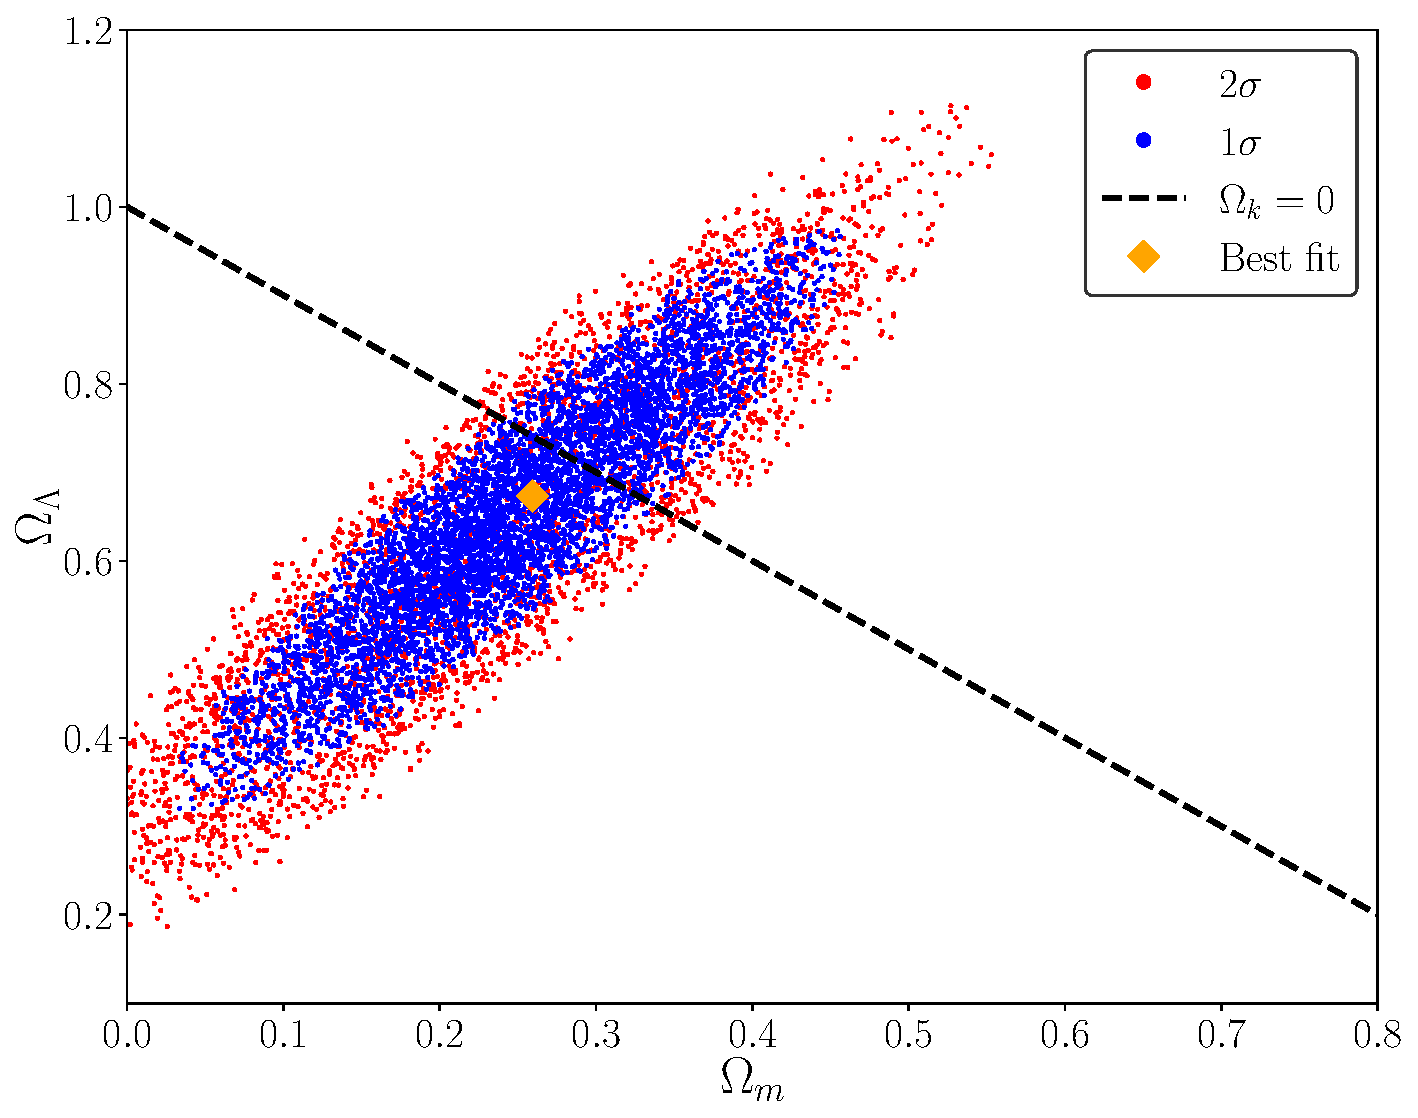
\includegraphics[width=\linewidth]{mcmc_supernova_fit_Nburn1000.pdf}
    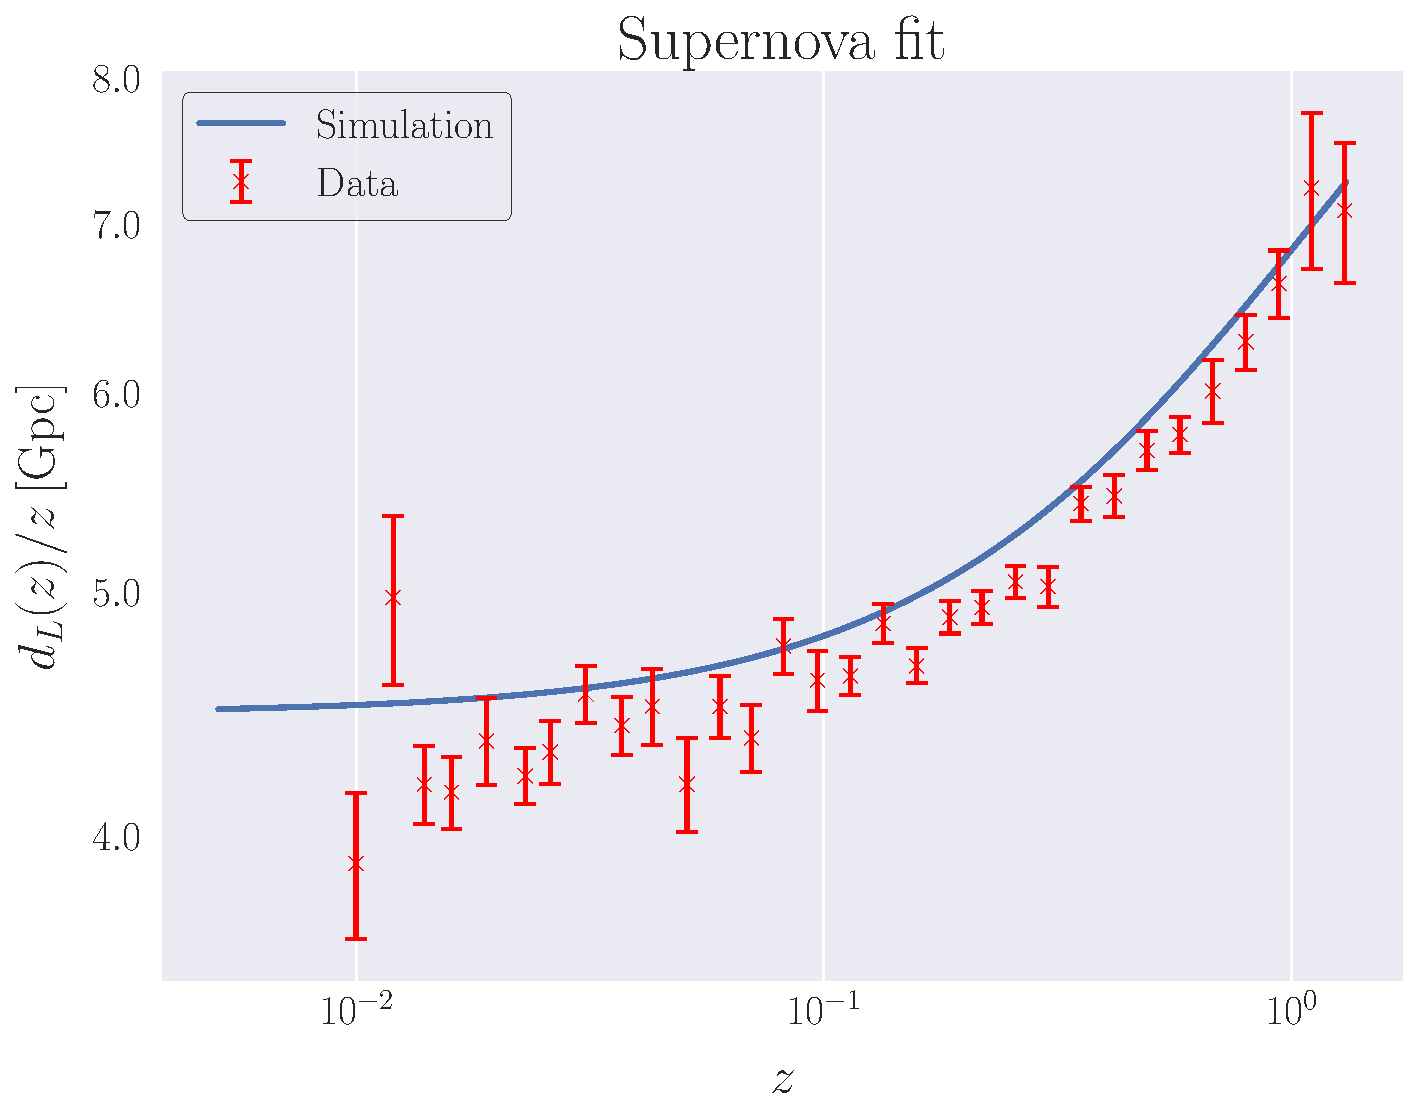
\includegraphics[width=\linewidth]{dL_z_compare_log.pdf}
\end{figure}